\section{OpenAI Gym}

The gym framework provides a standard definition of a reinforcement learning environment. It assumes that every environment is formalized with the Markov Decision Process (defined in section-\ref{section:markov}) \cite{OpenAIgym}. Hence, it follows the structure of the agent taking action and receiving observation and reward as a result of it.

\begin{figure}[htbp] 
    \centering
    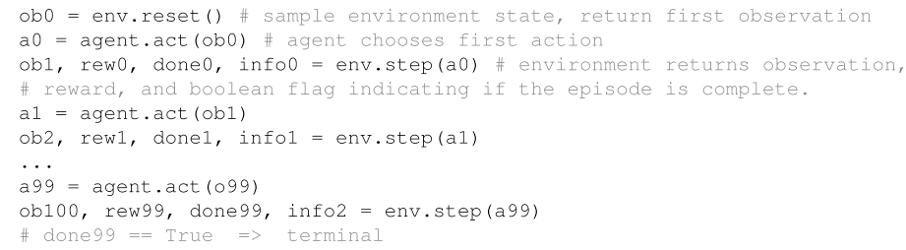
\includegraphics[width=1.0\textwidth]{figures/gyminterface}
    \caption{Gym interface to interact with an environment}
    \label{fig:gyminterface}
\end{figure}


The code example \ref{fig:gyminterface} demonstrates the interaction between an agent and the environment. OpenAI designed the Gym framework in a way that it is agent diagnostic. Therefore, it allows the user to try different algorithms on the agent side freely. The environment, on the other hand, should follow the Gym guidelines. A custom gym environment has to override the step, reset, seed, render, and close functions. The step function runs one timestep of the environment and returns a tuple of reward, observation, done, and info. The reset function resets the domain setting to a random or predefined initial state and returns the state's observation. The seed function starts the seeding of the random number generator. Close function is called at the end when the user wishes to quit the environment. Thus, it performs the necessary memory clean-up or resource deallocation.

\begin{lstlisting}[language=Python, caption=Gym environment example instantiation, label=gymexample]
    from gym.envs.registration import register

    register(
        id='gripper-env-v0',
        entry_point='manipulation_main.gripperEnv.robot:RobotEnv',
    )

    env = gym.make('gripper-env-v0', config='config/gripper_grasp.yaml')
\end{lstlisting}

Gym environment definition also provides a useful helper function gym.make(). After registering the custom environment, one can instantiate the environment with a simple one-liner represented in the code \ref{gymexample}. It also allows the user to pass an argument to the constructor of the custom environment. In our case, we provide the configuration file as an argument.